
\section{曲线上的应用}

现在，我们要把所学应用到\trCurve{}上。（这段讨论之所以来得这么晚，唯一的
原因是：我们需要\mbox{练习~16.2.G}，它蕴含若 $X\to Y$ 是\trFinite{}的，而 $Y$
在 $k$ 上射影，则 $X$ 在 $k$ 上也射影。）由于「\trCurve」一词可以有不同的含义，
我们在定理的陈述中将对假设力求一丝不苟。（在日常用法中，\trCurve{}常指%
\trPureDimension{} $1$ 的、某个\trField{} $k$ 上的\trVariety。）

\textbf{16.3.1.\ 定理（每条整\trCurve{}都有一个正则且射影的双有理模型）。}\ ——\
\emph{若 $C$ 是一个整的、有限型的、一维的 $k$-\trScheme，则存在正则射影的
$k$-\trVariety{} $C'$（维数为 $1$），与 $C$ 双有理。}

\emph{证明。}\quad 我们可以不妨设 $C$ 是\trAffine{}的。由\mbox{\trNoetherNormalization{}引理~12.2.4}，
我们可以找出某个 $x\in K(C)\setminus k$，使 $K(C)/k(x)$ 是一个\trFinite{}的\trFieldExtension。把
$\mathbb{P}^1_k$ 的一个\trStandardOpenSet{}等同于 $\Spec k[x]$，并在\trFunctionField{} $K(C)$
中取 $\mathbb{P}^1_k$ 的\trNormalization（定义见\mbox{练习~10.7.I}），我们便得到一个\trFinite\trMorphism
\[
C'\longrightarrow\mathbb{P}^1_k,
\]
其中 $C'$ 是一条\trCurve（\trFinite{}性由\mbox{练习~10.7.M}，$\dim C'=\dim\mathbb{P}^1_k$
由\mbox{练习~12.1.G}），并且正则（它既约，故在\trGenericPoint{}处正则；而在诸%
\trClosedPoint{}处，正则性由 \S13.5 中关于\trDVR{}的主定理给出）。此外，$C'$ 与 $C$
双有理，因为二者具有同构的\trFunctionField（\mbox{练习~7.5.E}）。

\begin{figure}[htbp]
\centering
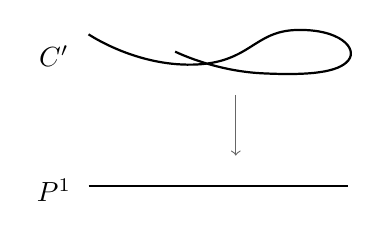
\begin{tikzpicture}[scale=1.1]
  \node at (-0.5,1.5) {$C'$};
  \draw[thick] plot [smooth, tension=1] coordinates {(-0.1,1.75) (1.1,1.4) (2.3,1.8) (2.9,1.45)
    (1.9,1.3) (0.9,1.55)};
  \draw[->, black!60] (1.6,1.05) -- (1.6,0.35);
  \draw[thick] (-0.1,0) -- (2.9,0);
  \node at (-0.5,-0.05) {$\mathbb{P}^1$};
\end{tikzpicture}
\caption{经 $\mathbb{P}^1$ 的一个有限覆盖，构造 $k$ 上\trCurve{} $C$ 的一个射影正则模型。
（依原书手绘图重绘。）}%
\label{fig:curve-proj-regular-model}
\end{figure}

最后，$C'\to\mathbb{P}^1_k$ 是\trFinite{}的，而 $\mathbb{P}^1_k\to\Spec k$ 是射影的，
于是由\mbox{练习~16.2.G}，$C'\to\Spec k$ 是射影的。\hfill$\square$

\textbf{16.3.2.\ 定理。}\ ——\ \emph{若 $C$ 是不可约、正则、一维的 $k$-\trVariety，则存在
一个\trOpenEmbedding{} $C\hookrightarrow C'$，其目标 $C'$ 是某条（$k$ 上的）射影正则\trCurve。}

\emph{证明。}\quad 我们先证 $C$ \trAffine{}的情形。与\mbox{定理~16.3.1} 的证明一样，我们有如下交换图
\[
\begin{tikzcd}[column sep=3.5em, row sep=3.5em]
C \ar[d, "\pi\ \text{有限}"'] & C' \ar[d, "\pi'\ \text{有限}"'] \\
\mathbb{A}^1_k \ar[r, hook] & \mathbb{P}^1_k,
\end{tikzcd}
\]
其中 $\pi'$ 是 $\mathbb{P}^1_k$ 在\trFunctionField{}扩张 $K(C)/K(\mathbb{A}^1_k)$ 中的\trNormalization，而
$C'$ 是射影的。由\trNormalization{}在\trFunctionField{}扩张中的\trUniversalProperty，$\mathbb{A}^1_k$ 在%
\trFunctionField{}扩张 $K(C)/K(\mathbb{A}^1_k)$ 中的\trNormalization{}正是 $C$ 本身，因为 $C$ 已经%
\trNormal。于是 $(\pi')^{-1}(\mathbb{A}^1_k)=C$，这便给出了想要的\trOpenEmbedding{}
$C\to C'$。

接下来我们考虑一般的 $C$。取 $C$ 的任意一个非空\trAffine\trOpenSubset{} $C_1$。由上一段的讨论，
我们有一个正则射影的\textbf{紧化}（compactification）$\widetilde{C}_1$。\mbox{曲线到射影的延拓定理~15.3.1}
（逐次应用于 $C\setminus C_1$ 的有限多个点）蕴含：\trMorphism{} $C_1\hookrightarrow\widetilde{C}_1$
可延拓为一个双有理\trMorphism{} $C\to\widetilde{C}_1$。由于\trSeparated{}正则\trCurve{}的点由其%
\trValuation{}所确定（\mbox{练习~13.7.B}），这便是集合论意义上的包含关系。又因为\trCurve{}上的拓扑是
「\trCofiniteTopology」，它把 $C$ 表为 $\widetilde{C}_1$ 的一个\trOpenSubset。但我们还没有大功告成！
\[
\begin{tikzcd}[column sep=3.5em, row sep=3.2em]
C_1 \ar[dr, hook] \ar[dd] & & \\
& C \ar[dl] & \\
\widetilde{C}_1 & &
\end{tikzcd}
\]
我们尚须证明：$C\to\widetilde{C}_1$ 是概形之间的\emph{\trOpenEmbedding}。为此，我们按如下方式证明它在任一点
$p$ 附近都是\trOpenEmbedding。取 $p$ 在 $C$ 中的一个\trAffine\trOpen\trNeighborhood{} $C_2$。
我们把在 $C_1$ 上用过的构造重演一遍，便得到下面这张标出了诸\trOpenEmbedding{}的交换图
\[
\begin{tikzcd}[column sep=2.8em, row sep=3.8em]
C_1 \ar[dr, hook] \ar[dd] & & C_2 \ar[dl, hook] \ar[dd] \\
& C \ar[dl] \ar[dr] & \\
\widetilde{C}_1 & & \widetilde{C}_2
\end{tikzcd}
\]
由\mbox{曲线到射影的延拓定理~15.3.1}，映射 $C_1\to\widetilde{C}_2$ 可延拓为
$\pi_{12}\colon\widetilde{C}_1\to\widetilde{C}_2$，而类似地我们也有一个\trMorphism{}
$\pi_{21}\colon\widetilde{C}_2\to\widetilde{C}_1$，延拓 $C_2\to\widetilde{C}_1$。复合
$\pi_{21}\circ\pi_{12}$ 是恒等\trMorphism（因为它是恒等\trRationalMap；见\mbox{定理~11.3.2}）。同理
$\pi_{12}\circ\pi_{21}$ 亦然，故 $\pi_{12}$ 与 $\pi_{21}$ 都是\trIsomorphism。于是加料后的交换图
\[
\begin{tikzcd}[column sep=2.8em, row sep=3.8em]
C_1 \ar[dr, hook] \ar[dd] & & C_2 \ar[dl, hook] \ar[dd] \\
& C \ar[dl] \ar[dr] & \\
\widetilde{C}_1 & & \widetilde{C}_2
\ar[ll, "\sim"]
\end{tikzcd}
\]
交换（仍是\mbox{定理~11.3.2}——它蕴含既约分离概形之间的\trMorphism{}由其在\trDense\trOpenSet{}上的
行为所确定）。但 $C_2\to\widetilde{C}_1$ 是一个\trOpenEmbedding（特别是在 $p$ 处），所以
$C\to\widetilde{C}_1$ 在 $p$ 处也是\trOpenEmbedding。\hfill$\square$

\textbf{16.3.A.（练习）}\quad 证明：$k$ 上所有正则的\trProper\trCurve{}都是射影的。

\textbf{16.3.3.\ 定理（\trCurve{}的种种范畴是同一个）。}\ ——\ \emph{以下诸\trCategory{}等价：}

（i）\emph{整的、正则的、射影的一维 $k$-簇，以及满的 $k$-\trMorphism；}

（ii）\emph{整的、正则的、射影的一维 $k$-簇，以及支配的 $k$-\trMorphism；}

（iii）\emph{整的、正则的、射影的一维 $k$-簇，以及支配的 $k$ 上\trRationalMap；}

（iv）\emph{整的、一维的 $k$-簇，以及支配的 $k$ 上\trRationalMap；}以及

（v）\emph{「在 $k$ 上超越次数为 $1$ 的有限生成域，连同 $k$-同态」这一\trCategory{}的%
\trOppositeCategory（定义见 \S1.1.16）。}

在下面的讨论中，一切\trMorphism{}与\trMap{}都默认定义在 $k$ 上。

（旁注：有兴趣的读者可以微调下面的证明，来证明本定理的下述变体。在（i）--（iv）中，只考虑%
\trGeometricallyIrreducible{}的\trCurve；而在（v）中，只考虑满足「在 $\overline{k}$ 中
$K\cap k^s=k$」的域 $K$。这一变体使我们能够排除那些我们未必想考虑的「怪异」\trCurve。例如，
若 $k=\mathbb{R}$，那么我们便允许了诸如 $\mathbb{P}^1_{\mathbb{C}}$ 这类非%
\trGeometricallyIrreducible{}的\trCurve，因为
$\mathbb{P}^1_{\mathbb{C}}\times_{\mathbb{R}}\Spec\mathbb{C}\cong
\mathbb{P}^1_{\mathbb{C}}\amalg\mathbb{P}^1_{\mathbb{C}}$。）

\emph{证明。}\quad 每个满态射都是支配态射，而每个支配态射都是支配有理映射，又每条整的正则射影%
\trCurve{}都是拟射影\trCurve，于是我们已（不严格地说）展示了如何从（i）走到（ii）再走到（iii）
最后走到（iv）。要从（iv）走到（i），设我们有一条整\trCurve{}之间的支配\trRationalMap{}
$C_1\dashrightarrow C_2$。把 $C_1$ 换成一个\trDense\trOpenSet，使该\trRationalMap{}成为一个%
\trMorphism{} $C_1\to C_2$。这诱导出正则不可约\trCurve{}的\trNormalization{}之间的一个映射
$\widetilde{C}_1\to\widetilde{C}_2$。取 $\overline{\widetilde{C}}_i$ 为 $\widetilde{C}_i$ 的一个正则
射影紧化（$i=1,2$），如\mbox{定理~16.3.2} 中那样。于是，由
\mbox{曲线到射影的延拓定理~15.3.1}，\trMorphism{} $\widetilde{C}_1\to\widetilde{C}_2$ 可延拓为%
\trMorphism{} $\overline{\widetilde{C}}_1\to\overline{\widetilde{C}}_2$。这个\trMorphism{}是满的
（你看出缘由了吗？），于是我们便在范畴（i）中造出了一个\trMorphism。

\textbf{16.3.B.（练习）}\quad 把上面的各个部件拼装起来，具体描述范畴（i）至（iv）的等价。

剩下的只是把（v）也接上。这本质上就是\mbox{练习~7.5.E} 的内容；细节留给读者。\hfill$\square$

\mbox{定理~16.3.3} 有好些个推论。例如，每条既约的拟射影\trCurve{}都恰与唯一一条射影正则%
\trCurve{}双有理。下面是另一个有意思的推论。

\textbf{16.3.4.\ 重要观念：从\trCurve{}到正则\trCurve{}的射影态射的次数。}

对于紧致\trRiemann{}曲面之间的映射有一个表现良好的次数——只要以恰当的重数清点原像，$C'$ 的
一个点的原像个数便为常数——你或许已有相当合理的直觉。例如，若 $f$ 局部看起来像
$z\mapsto z^m=y$，那么在 $y=0$ 与 $z=0$ 附近（但不在 $z=0$ 处），每个点都恰有 $m$ 个原像；
而当 $y$ 趋于 $0$ 时，这 $m$ 个原像便并合起来。富有启发性的\mbox{例~10.3.4} 已在一个
更复杂的情境中展示过这个现象。

现在我们来证明这个事实的代数版本。设 $\pi\colon C\to C'$ 是正则射影\trCurve{}之间的一个满
（等价地，支配）映射。我们将证明 $\pi$ 有一个表现良好的次数，其确切含义我们现在就来厘定。

我们先证 $\pi$ 是\trFinite{}的。\mbox{定理~18.1.6}（有限＝射影＋有限\trFiber）蕴含这一点，
但我们还没有证明它。于是，作为替代，我们按如下方式证明 $\pi$ 的\trFinite{}性。取 $C''$ 为
$C'$ 在 $C$ 的\trFunctionField{}中的\trNormalization。那么我们有同构
$K(C)\cong K(C'')$（实际上就是相等），它诱导出双有理映射
$C\mathrel{\leftharpoonup\joinrel\relbar\joinrel\rightharpoondown}C''$；由于 $C$ 与 $C''$ 都
正则且射影，这些映射可延拓为\trMorphism（由\mbox{曲线到射影的延拓定理~15.3.1}）。于是这就给出了
$C$ 与 $C''$ 的一个\trIsomorphism。而由\trNormalization{}的\trFinite{}性
（\mbox{练习~10.7.M}），$C''\to C'$ 是\trFinite\trMorphism。

\textbf{16.3.5.\ 命题。}\ ——\ \emph{设 $\pi\colon C\to C'$ 是一个\trFinite\trMorphism，其中
$C'$ 是\trPureDimension{} $1$ 的正则\trNoetherian\trScheme，而 $C$ 是\trPureDimension{} $1$
且无\trEmbeddedPoint{}的\trNoetherian\trScheme（最重要的情形：$C$ 既约）。那么 $\pi_*\OO_C$
是有限秩的\trLocallyFreeSheaf。}

「无\trEmbeddedPoint」这一假设，等价于要求 $C$ 的每个\trAssociatedPoint{}都映到（$C'$ 的某个
不可约分量的）\trGenericPoint{}上。注意：若 $C$ 既约，则 $C$ 的奇点可以糟糕到什么程度完全不受
限制！

我们将在 \S16.3.11 中证明\mbox{命题~16.3.5}，在那之前先展示它何等有用。$C'$ 上的正则性假设是
必要的：结点曲线（\cref{fig:normalization-nodal-cubic}）的\trNormalization{}便是一例——大多数
点只有一个原像，而有一个点（「\trNode」）却有两个。（在\mbox{注记~24.3.8} 与 \S24.3.12 中我们
将会看到，\mbox{命题~16.3.5} 的诸假设中真正要紧的，是该\trMorphism{}既\trFinite{}又\trFlat。）

\textbf{16.3.6.}\ \emph{\trhDefinition{}。}\quad 若 $C'$ 不可约，则这个\trLocallyFreeSheaf{}的
秩就称为 $\pi$ 的\textbf{\trDegree}。

\textbf{16.3.C.（练习）}\quad 回想：从一条整\trCurve{}到另一条整\trCurve{}的\trRationalMap{}的%
\trDegree{}定义为\trFunctionField{}扩张的\trDegree（\mbox{定义~12.2.2}）。证明：在
\mbox{命题~16.3.5} 的记号下，若 $C$ 与 $C'$ 都是整的，则作为\trRationalMap{}的 $\pi$ 的%
\trDegree{}与 $\pi_*\OO_C$ 的秩相同。

\textbf{16.3.7.}\ \emph{写给具有复解析背景的读者的注记（代数\trDegree{}＝解析\trDegree）。}\quad
若 $C\to C'$ 是正则的复代数\trCurve{}之间的一个\trFinite{}映射，则\mbox{命题~16.3.5} 建立了：
上面定义的代数\trDegree{}与解析\trDegree{}相同（以重数清点原像）。

\textbf{16.3.D.（练习）}\quad 我们沿用\mbox{命题~16.3.5} 的记号与假设。设 $p$ 是 $C'$ 的一个%
\trClosedPoint。$p$ 的概形论原像 $\pi^{-1}(p)$ 是 $k$ 上的一个维数 $0$ 的\trScheme。
（a）设 $C'$ 在某个\trField{} $k$ 上有限型，并设 $n$ 是 $\pi^{-1}(p)$ 的\trStructureSheaf{}的%
\trGlobalSections{}所构成的 $k$-\trVectorSpace{}的\trDimension。证明：
$n=(\deg\pi)(\deg p)$。（点的\trDegree{}定义于 \S5.3.8。）
（b）设 $C$ 正则，并且 $\pi^{-1}(p)=\{p_1,\dots,p_m\}$。设 $t$ 是\trDVR{} $\OO_{C',p}$ 的一个%
\trUniformizer。证明：
\[
\deg\pi=\sum_{i=1}^{m}(\mathrm{val}_{p_i}\,\pi^*t)\,\deg(\kappa(p_i)/\kappa(p)),
\]
其中 $\deg(\kappa(p_i)/\kappa(p))$ 表示剩余域之\trFieldExtension{}的次数。（你能推广（a），把
「在域上工作」的假设去掉吗？如果你是数论工作者，你能用「数域的整数环之扩张中素理想的分裂」的
语言辨认出（b）吗？）

\textbf{16.3.E.（练习）}\quad 设 $C$ 是 $k$ 上一条不可约正则射影\trCurve，而 $s$ 是 $C$ 上的一个非零%
\trRationalFunction。证明：$s$ 的\trZeros{}的个数（以恰当的重数清点）等于其\trPole{}的个数。提示：
把这认作\trMorphism{} $s\colon C\to\mathbb{P}^1_k$ 的次数。对 $0\in\mathbb{P}^1$ 与
$\infty\in\mathbb{P}^1$ 两个情形使用\mbox{练习~16.3.D}(b)。（在复范畴中，这是留数定理的一个重要
推论。）

\textbf{16.3.8.}\ \extrahard\ \emph{一个现在就能作出的重要定义（尽管我们要等到 \S18.4.2）。}\quad
写到这里，我们其实已经能够轻而易举地作出「\trSmooth{}射影\trCurve{}上的\trLineBundle{}的%
\trDegree{}」这一重要定义了。你不妨现在就把它想通，尽管我们要等到 \S18.4.2 才作出一个
（貌似不同的）定义，并在\mbox{重要容易练习~18.4.C} 中证明它与这个定义等价。设 $C$ 是 $k$
上一条不可约正则射影\trCurve，而 $\mathscr{L}$ 是 $C$ 上的一个\trLineBundle。那么
$\mathscr{L}$ 便拥有一个非零\trRational\trSection{} $s$（你看出缘由了吗？）。若 $s$ 与
$t$ 是任意两个非零\trRational\trSection，则由\mbox{练习~16.3.E}，对\trRationalFunction{}
$s/t$ 而言，零点的个数等于极点的个数（正确清点）\footnote{原书此处作「for the the
rational function」，当为「for the rational function」之误，径改。——译者注}。于是，非零%
\trRational\trSection{} $s$ 的「零点个数减去极点个数」（正确清点）不依赖于 $s$ 的选取。
这个整数本可以被取作\trCurve{} $C$ 上\trLineBundle{} $\mathscr{L}$ 的\trDegree{}的定义。
（由于我们并未把它当作「正式定义」，我们就不把这个短语排成粗体。）

\textbf{16.3.9.}\ \emph{\trhRemark{}。}\quad 在\mbox{练习~18.4.E} 中，我们将会看到：上一练习
中零点（与极点）的个数，正是给出到 $\mathbb{P}^1$ 之映射的那个\trLineBundle{}的%
\trDegree（经由\mbox{重要定理~15.2.2}）。

\textbf{16.3.10.}\ \emph{重温\mbox{例~10.3.4}。}\quad \mbox{命题~16.3.5} 与\mbox{练习~16.3.D}
把我们在\mbox{例~10.3.4} 中观察到的一般行为精确化了。设 $C'$ 不可约，并设 $d$ 是这个号称%
\trLocallyFreeSheaf{}的东西的秩。那么，$C'$ 的任一个\trResidueField{}为 $K$ 的点上的%
\trFiber，都是某个 $K$ 上维数为 $d$ 的\trAlgebra{}的 $\Spec$。这意味着\trFiber{}中点的
个数（以恰当的重数清点）总是 $d$。

作为一个动机性的例子，我们重温\mbox{例~10.3.4}：由 $x\mapsto y^2$ 给出的映射
$\mathbb{Q}[y]\to\mathbb{Q}[x]$\footnote{原书此处作「the map $\mathbb{Q}[y]\to\mathbb{Q}[x]$
given by $x\mapsto y^2$」——按「$x\mapsto y^2$」读法，环映射的方向当为
$\mathbb{Q}[x]\to\mathbb{Q}[y]$（\mbox{例~10.3.4} 原文正是如此），此处箭头疑当为笔误，
兹照录原书。——译者注}，即\trParabola{} $x=y^2$ 到 $x$-轴的\trProjection。我们当时观察到
如下现象。
（i）$x=1$ 之上的\trFiber{}是 $\mathbb{Q}[y]/(y^2-1)$，于是我们得到 $2$ 个点。
（ii）$x=0$ 之上的\trFiber{}是 $\mathbb{Q}[y]/(y^2)$——我们得到一个点，重数为 $2$，
起因于非既约性。
（iii）$x=-1$ 之上的\trFiber{}是 $\mathbb{Q}[y]/(y^2+1)\cong\mathbb{Q}(i)$——我们得到一个
点，重数为 $2$，起因于\trFieldExtension。
（iv）最后，\trGenericPoint{} $\Spec\mathbb{Q}(x)$ 之上的\trFiber{}是 $\Spec\mathbb{Q}(y)$，
这是一个点，重数为 $2$，同样起因于\trFieldExtension（因为 $\mathbb{Q}(y)/\mathbb{Q}(x)$
是 $2$ 次的\trFieldExtension）。
于是我们看到三种行为（其中情形（iii）与（iv）实为同一回事）。注意：即便你只在%
\trAlgClosedField{}上工作，你仍然会被迫去对付这第三种行为，因为\trGenericPoint{}处的%
\trResidueField{}通常不\trAlgClosed（上面的情形（iv）便是明证）。

\textbf{16.3.11.}\ \emph{\mbox{命题~16.3.5} 的证明。}\quad 其中的关键想法——它在别的场合也有
用——是化归到关于\trDVR{}的一个事实。

这个问题在靶上是局部的，故不妨设 $C'$ 是\trAffine{}的。如今 $C'$ 是\trNormal{}的，于是由
\mbox{练习~5.4.B}，它的诸\trConnectedComponent{}都不可约。把 $C'$ 换成它的每一个%
\trIrreducibleComponent，我们还不妨设 $C'$ 是整的。

由\mbox{练习~14.3.K}，若有限型\trQCSheaf{} $\pi_*\OO_C$ 的秩是常数，则（由于 $C'$ 既约）
$\pi_*\OO_C$ 是\trLocallyFree{}的。我们将这样来证明它：证明 $C'$ 在任一\trClosedPoint{} $p$
处的秩与它在\trGenericPoint{}处的秩相同。（这是\trGenericPoint{}之有用性的又一个例子。）

设 $C'=\Spec A'$，其中 $A'$ 是一个\trIntegralDomain，并设 $p=[\mathfrak{m}]$。由于 $\pi$
是\trAffine\trMorphism，$C$ 也是\trAffine\trScheme；比如说，$C=\Spec A$。

我们希望证明：（i）$\dim_{A'/\mathfrak{m}}(A/\mathfrak{m})$（$\pi_*\OO_C$ 在 $p$ 处的秩）
等于（ii）$\dim_{K(A')}(A'^\times)^{-1}A$（$\pi_*\OO_C$ 在\trGenericPoint{}处的秩）。换个
话说，我们取 $A$（视作一个 $A'$-\trModule），然后（i）模掉 $\mathfrak{m}$，（ii）把 $A'$
的全部非零元都取逆，再在每种情形下计算所得者在相应\trField{}上的维数。

（i）与（ii）都穿过在 $\mathfrak{m}$ 处的\trLocalization{}分解，故只需证明：
$A_{\mathfrak{m}}$ 是一个秩有限的自由 $A'_{\mathfrak{m}}$-\trModule，比如说秩为 $d$——
因为届时（i）与（ii）的答案都将是 $d$。

如今 $A'_{\mathfrak{m}}$ 是一个\trDVR；设 $t$ 是它的\trUniformizer。我们可以假设
$t\in A'$（因为不然的话，我们就把 $A'$ 换成一个适当的\trLocalization，即在 $t$ 的诸
「分母」处取局部化）。此时 $A_{\mathfrak{m}}$ 是有限生成的 $A'_{\mathfrak{m}}$-\trModule，
从而由\mbox{注记~6.4.4}，它是\trPrincipalModule（principal module）的有限\trDirectSum，形状为 $A'_{\mathfrak{m}}$
或 $A'_{\mathfrak{m}}/(t^n)$（$n$ 取各种值）。我们希望证明：后一类型的直和项并不出现。
但倘若出现，则 $t$（解释为 $A_{\mathfrak{m}}$ 中的元素）将是 $A_{\mathfrak{m}}$ 的一个%
\trZerodivisor，从而（解释为 $A$ 中的元素）是 $A$ 的\trZerodivisor。但那样一来，由
\mbox{命题~6.6.13}，在 $\pi^{-1}(p)$ 中便有 $C$ 的一个\trAssociatedPoint，这与「$C$
无\trEmbeddedPoint」的假设相矛盾。\hfill$\square$

